% !TEX program = xelatex
\documentclass[zihao=-4,a4paper]{ctexart}
\usepackage{fontspec}
\usepackage{xeCJK}
\usepackage{amsmath,amssymb,bm}
\usepackage{graphicx}
\usepackage{listings}
\usepackage{xcolor}
\usepackage{float}
\usepackage{enumitem}
\usepackage{caption}
\usepackage{booktabs}
\usepackage{array}
\usepackage{algorithm}
\usepackage{algpseudocode}
\usepackage{changepage} % 用于调整局部正文的左右边距
\usepackage{pdfpages}
\setmonofont{Consolas}   % 设置等宽字体为 Consolas
\setCJKmainfont{SimSun}[AutoFakeBold=2.5]
\usepackage{hyperref}
% 页面布局
\usepackage[
  top    = 1.7cm,
  left   = 1.7cm,
  right  = 1.7cm,
  bottom = 2.7cm,
  footskip = 1cm
]{geometry}
\linespread{1.5}
% 提供 current page text area 节点
\usepackage{tikzpagenodes}
\usetikzlibrary{calc}            % 用于计算坐标
\usepackage{fancyhdr}
% ==============================
% 全局变量: 存储版心宽度
% ==============================
\newlength{\myTextWidth}
\newcommand{\calcTextWidth}{%
  \path let \p1=(current page text area.east), \p2=(current page text area.west) in 
    \pgfextra{\pgfmathsetlength{\myTextWidth}{\x1-\x2}};
}

% ==============================
% 背景画线逻辑
% ==============================
\newif\ifdrawbackground  % 定义背景绘制开关
\drawbackgroundtrue      % 默认开启背景绘制
\AddToHook{shipout/background}{%
  \ifdrawbackground %只有开关开启时才绘制背景
  \tikz[remember picture, overlay]{%
    
    % 定义上下外扩的距离(和表格撑开的距离保持一致)
    \def\vpad{0.8em} 

    % --- 所有页: 底部横线 (向下偏移 \vpad) ---
    \draw[line width=1pt] 
      ([yshift=-\vpad]current page text area.south west) -- 
      ([yshift=-\vpad]current page text area.south east);

    \ifnum\value{page}=1
      % --- 第一页: 绘制 2x6 表格边框 ---
      \def\innerLineWidth{0.8pt}
      \def\outerLineWidth{1pt}

      % 1. 上横线 (表格节点已通过 inner ysep 撑开, 直接画)
      \draw[line width=\outerLineWidth] 
        (title-bottom-mark -| current page text area.west) -- 
        (title-bottom-mark -| current page text area.east);

      % 2. 下横线 (同上)
      \draw[line width=\outerLineWidth] 
        (table-bottom-mark -| current page text area.west) -- 
        (table-bottom-mark -| current page text area.east);

      % 3. 中间横线 (自动居中)
      \draw[line width=\innerLineWidth] 
        ($(title-bottom-mark -| current page text area.west)!0.5!(table-bottom-mark -| current page text area.west)$) -- 
        ($(title-bottom-mark -| current page text area.east)!0.5!(table-bottom-mark -| current page text area.east)$);

      % 4. 左右外框竖线 (从表格顶部一直到页底, 页底向下偏移 \vpad)
      \draw[line width=\outerLineWidth] 
        (title-bottom-mark -| current page text area.west) -- 
        ([yshift=-\vpad]current page text area.south west);
      \draw[line width=\outerLineWidth] 
        (title-bottom-mark -| current page text area.east) -- 
        ([yshift=-\vpad]current page text area.south east);

      % 5. 内部竖线 (5条)
      \foreach \i in {1,2,...,5} {
        \pgfmathsetmacro{\pos}{\i/6}
        \draw[line width=\innerLineWidth]
          ($(title-bottom-mark -| current page text area.west)! \pos !(title-bottom-mark -| current page text area.east)$) --
          ($(table-bottom-mark -| current page text area.west)! \pos !(table-bottom-mark -| current page text area.east)$);
      }

    \else
      % --- 后续页: 标准四周边框 (上下各外扩 \vpad) ---
      % 顶部横线向上偏移
      \draw[line width=1pt] ([yshift=\vpad]current page text area.north west) -- ([yshift=\vpad]current page text area.north east);
      % 左右竖线跟随上下偏移
      \draw[line width=1pt] ([yshift=\vpad]current page text area.north west) -- ([yshift=-\vpad]current page text area.south west);
      \draw[line width=1pt] ([yshift=\vpad]current page text area.north east) -- ([yshift=-\vpad]current page text area.south east);
    \fi
  }%
  \fi
}


\pagestyle{fancy}
\fancyhf{}
\fancyfoot[C]{\thepage}
\renewcommand{\headrulewidth}{0pt}

% 直接使用 \textwidth 计算列宽
% ==============================
% \textwidth/6 保证精确6等分, 减去 2\tabcolsep 扣除单元格自带的左右边距
\newcolumntype{C}{>{\raggedright\arraybackslash}p{\dimexpr\textwidth/6-2\tabcolsep\relax}}

% 自定义命令: 在当前位置画一条贯穿全宽的横线
% ==============================
\newcommand{\addhline}{%
  \par
  \noindent
  
\begin{tikzpicture}[remember picture, overlay]
    % (0,0) 代表当前文字所在的高度
    % current page text area.west 代表版心最左侧
    % |- 符号表示: 取左边的 X 坐标, 取右边的 Y 坐标
    \draw[line width=1pt] 
      (current page text area.west |- 0,0) -- 
      (current page text area.east |- 0,0);
  \end{tikzpicture}\par
}

\newcommand{\dd}{\mathop{}\!\mathrm{d}}
\newcommand{\myS}{14}
\newcommand{\myt}{0.21}

% MATLAB 代码风格
\definecolor{matlabgreen}{rgb}{0,0.6,0}
\definecolor{matlabgray}{rgb}{0.5,0.5,0.5}
\definecolor{matlabpurple}{rgb}{0.58,0,0.82}
\definecolor{matlabbg}{rgb}{0.95,0.95,0.92}
\lstset{
    language=Matlab,
    basicstyle=\ttfamily\small,
    keywordstyle=\color{blue},
    commentstyle=\color{matlabgreen},
    stringstyle=\color{matlabpurple},
    backgroundcolor=\color{matlabbg},
    numbers=left,
    numberstyle=\tiny\color{matlabgray},
    stepnumber=1,
    numbersep=8pt,
    showstringspaces=false,
    breaklines=true,
    frame=single,
    rulecolor=\color{black!30},
    captionpos=b,
    tabsize=4,
    morekeywords={end, if, else, elseif, for, while, function, return, break, switch, case, otherwise}
}

\begin{document}

% 插入封面: 临时关闭背景绘制 + 清空页眉页脚 + 不占页码
\drawbackgroundfalse
\pagestyle{empty}
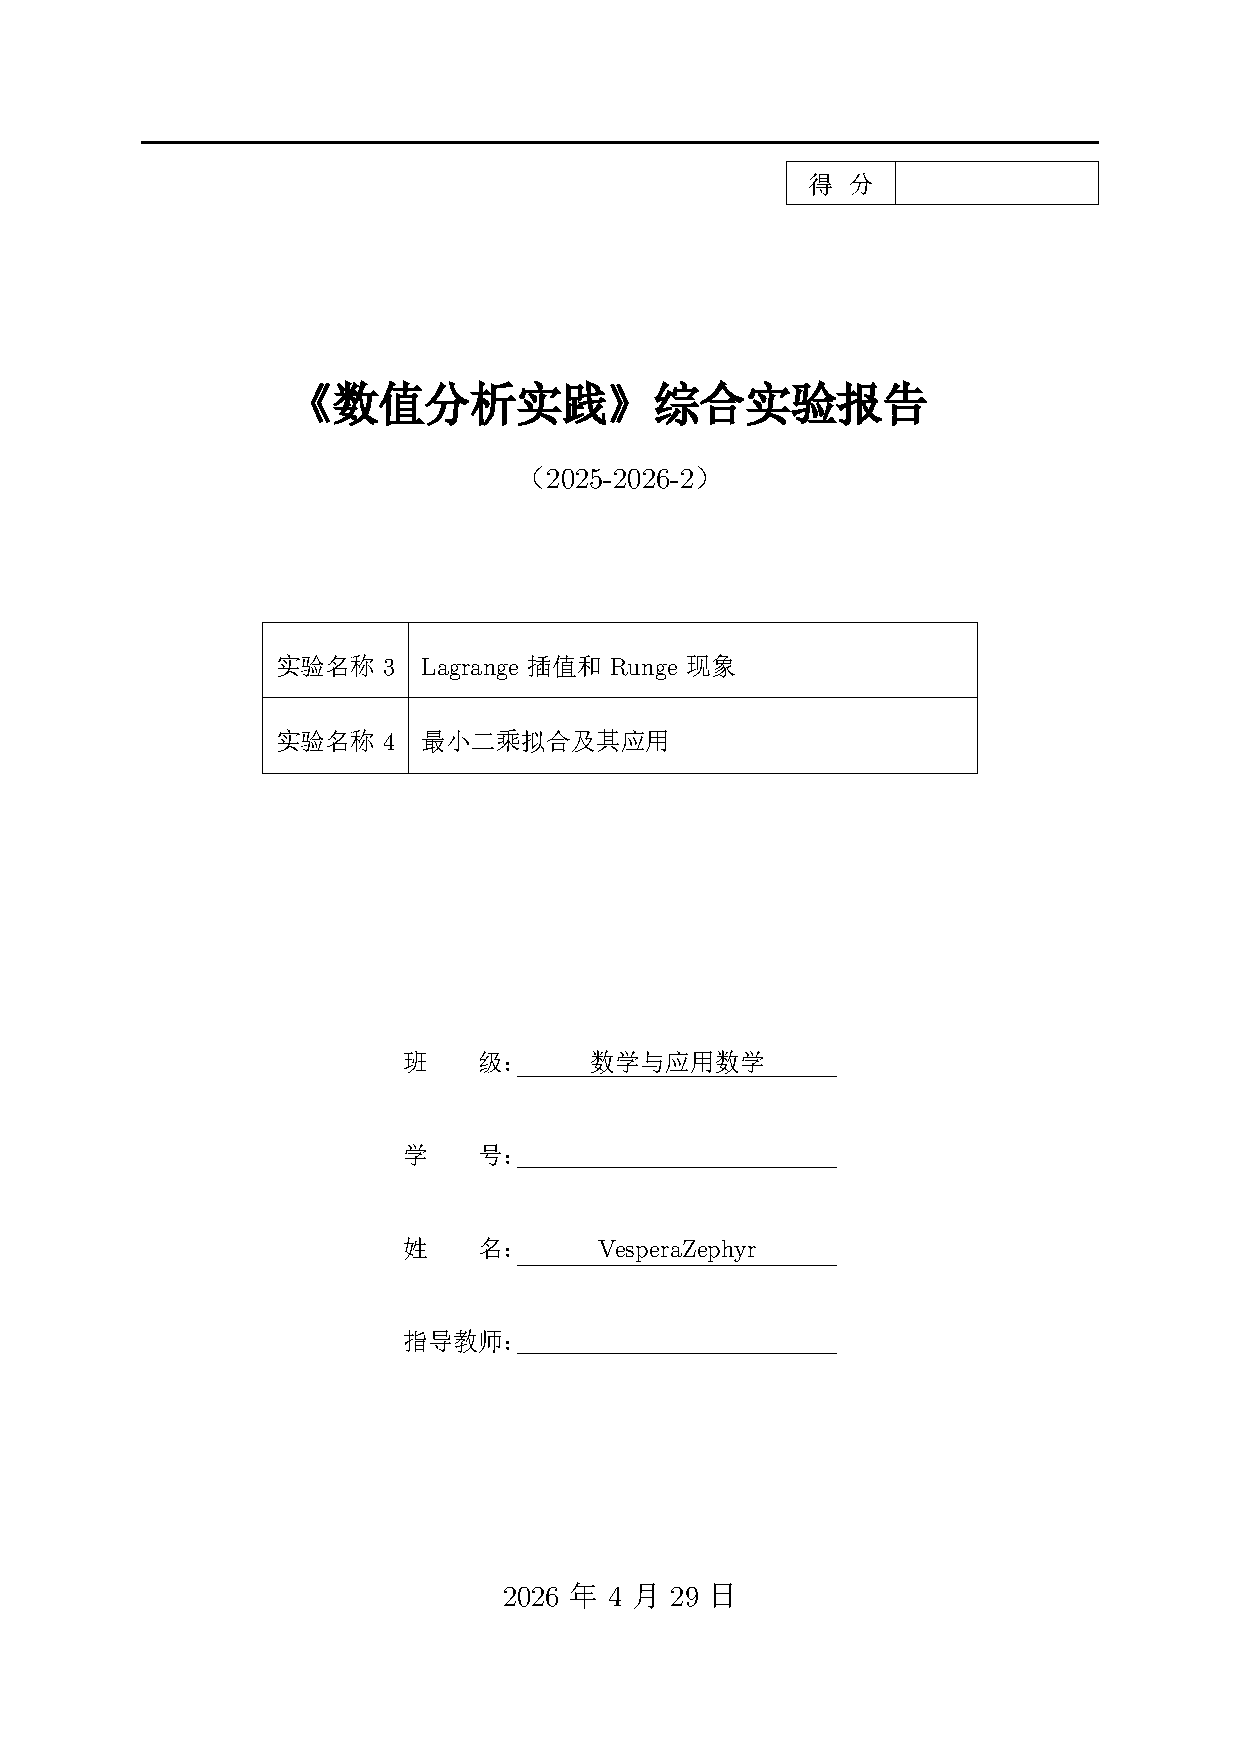
\includepdf[pages={1}]{封面.pdf}
\drawbackgroundtrue  % 恢复背景绘制
\pagestyle{fancy}    % 恢复你的页眉页脚
\setcounter{page}{1} % 重置页码, 正文从第1页开始(完美兼容你原来的 \ifnum\value{page}=1 逻辑)

\begin{center}
  \zihao{-2}\bfseries 数值分析实践报告(三)
\end{center}

% --- 表格内容区 ---
\noindent
\begin{tikzpicture}[remember picture]
  % 将整个 tabular 放入一个 TikZ 节点中, 彻底屏蔽 LaTeX 段落间距的干扰
  \node[anchor=north west, inner sep=0pt, outer sep=0pt] (header-table) at (0,0) {%
    \renewcommand{\arraystretch}{1.8}% 增加行高
    \begin{tabular}{CCCCCC} 
      姓\quad 名 & VesperaZephyr & 班\quad 级 & \small 数学与应用数学 & 报告评分 & \\
      学\quad 号 & 114514 & 地点/机号 &  & 指导教师 & 
    \end{tabular}%
  };
  
  % 自动获取这个表格真实的左上角和左下角坐标, 传给背景画线
  \coordinate (title-bottom-mark) at (header-table.north west);
  \coordinate (table-bottom-mark) at (header-table.south west);
\end{tikzpicture}

\setlength{\leftskip}{1em}
\setlength{\rightskip}{1em}

% 实验名称
\noindent{\bfseries 一、实验项目名称: Lagrange插值和Runge现象}

\addhline

\noindent{\bfseries 二、实验目的: }
\begin{enumerate}
  \item 底层构建: 理解拉格朗日插值基函数的数学原理. 
  \item 算法实践: 掌握拉格朗日插值的算法和代码. 
  \item 现象观察: 观察并分析高次插值中的 Runge 现象(边缘震荡)
  \item 根源探究: 通过分析余项来揭示Runge现象的本质. 
  \item 策略优化: 学习使用Chebyshev节点(极值点)抑制震荡. 
\end{enumerate}

\addhline

\noindent{\bfseries 实验内容: }

给定 $n+1$ 个插值节点, Lagrange插值多项式的定义为
\[
P_n(x)=\sum_{i=0}^{n} y_i \, l_i(x)
\]
其中基函数 $l_i(x)$ 的表达式为
\[
l_i(x)=\prod_{\substack{j=0 \\ j\neq i}}^{n} \frac{x-x_j}{x_i-x_j}, \quad i=0,1,2,\dots,n
\]
考虑函数 $\displaystyle y=f(x)=\frac{1}{1+25x^{2}},\ x\in[-1,1]$, 

取等距插值节点为 $\displaystyle x_i=-1+\frac{2i}{n},\ i=0,1,2,\dots,n$, $y_i=f(x_i)$
\[
\begin{array}{c|c|c|c|c}
x_0 & x_1 & x_2 & \cdots & x_n \\
\hline
y_0 & y_1 & y_2 & \cdots & y_n
\end{array}
\]

\noindent\textbf{第一阶段: 基函数与插值算法构造}

\noindent\textbf{任务1\quad 编写基函数计算器}

给定 $n,\ i,\ x$, 编写函数计算基函数 $l_i(x)$ 在点 $x$ 处的值。

\noindent\textbf{任务2\quad 实现插值函数}

利用任务1的结果, 计算完整的多项式 $P_n(x)$ 在点 $x$ 处的值。

\noindent\textbf{第二阶段: Runge现象的观察}

\noindent\textbf{任务1\quad 边缘误差的爆炸趋势}

\begin{itemize}[rightmargin=0.5cm]
  \item 在区间 $[-1,1]$ 内, 分别取 $n=3,5,8,10,15,20$。若给定 $x=0.91$, 计算 $P_n(x)$ 的值, 计算误差 $|P_n(x)-f(x)|$。
  \item 画出该误差随着 $n$ 的变化曲线。
\end{itemize}

\noindent\textbf{任务2\quad } 取 $n=20$, 画出 $P_n(x)$ 的曲线, 和 $f(x)$ 的曲线相比, 你有什么发现？

\addhline

\noindent{\bfseries 四、模型构建}

给定 $n+1$ 个互异的插值节点 $(x_i, y_i), i=0,1,\dots,n$, 其中 $y_i=f(x_i)$, Lagrange插值多项式定义为
\begin{equation}
    P_n(x) = \sum_{i=0}^{n} y_i \cdot l_i(x)
    \label{eq:lagrange}
\end{equation}
基函数 $l_i(x)$ 的表达式为
\begin{equation}
    l_i(x) = \prod_{\substack{j=0\\ j\neq i}}^{n} \frac{x-x_j}{x_i-x_j},\quad i=0,1,\dots,n
    \label{eq:basis}
\end{equation}
本实验选择函数
\begin{equation}
    f(x) = \frac{1}{1+25x^2},\quad x\in[-1,1]
\end{equation}
并采用等距节点
\begin{equation}
    x_i = -1 + \frac{2i}{n},\quad i=0,1,\dots,n
\end{equation}
计算对应的 $y_i = f(x_i)$, 构造插值多项式 $P_n(x)$. 

\addhline

\noindent{\bfseries 五、模型求解}

\noindent{\bfseries 第一阶段: 基函数与插值算法构造}

\noindent{\bfseries 任务1\quad 编写基函数计算器}

算法步骤为
\begin{center}
  \begin{minipage}{0.8\textwidth}
    \begin{algorithm}[H]
  \caption{计算 Lagrange 插值基函数 $l_i(x)$ 的值}
    \begin{algorithmic}[1]
      \Require 等分份数 $n$(节点数为 $n+1$), 基函数下标 $i$($0 \le i \le n$), 求值点 $x$(标量或向量)
      \Ensure $L = l_i(x)$, 与 $x$ 尺寸相同
      \State 生成等距节点: $x_j = -1 + \dfrac{2j}{n}$, $j = 0,1,\dots,n$
      \State 令 $idx = i + 1$(转换为 MATLAB 下标, 用于访问节点数组)
      \State 初始化 $L \gets \mathbf{1}$(与 $x$ 同尺寸的全 1 向量/标量)
      \For{$k = 1$ 至 $n+1$}
          \If{$k \neq idx$}
              \State $L \gets L \cdot \dfrac{x - x_k}{x_{idx} - x_k}$(逐元素乘法)
          \EndIf
      \EndFor
      \Return $L$
    \end{algorithmic}
  \end{algorithm}
  \end{minipage}
\end{center}


据此编写Matlab函数\verb|lagrange_basis.m|, 输入参数为 $n$、$i$ 和 $x$, 输出为 $l_i(x)$ 的值.

\noindent\textbf{任务2\quad 实现插值函数}

算法步骤为
\begin{center}
  \begin{minipage}{0.8\textwidth}
    \begin{algorithm}[H]
    \caption{基于等距节点的 Lagrange 插值多项式求值}
      \begin{algorithmic}[1]
        \Require 等分份数 $n$, 求值点 $x$(标量或向量), 被插函数 $f(x)=\dfrac{1}{1+25x^2}$, 区间 $[-1,1]$
        \Ensure $P = P_n(x)$, 与 $x$ 尺寸相同
        \State 生成等距节点: $x_j = -1 + \dfrac{2j}{n}$, $j = 0,1,\dots,n$
        \State 计算节点函数值: $y_j = f(x_j) = \dfrac{1}{1+25x_j^2}$, $j = 0,1,\dots,n$
        \State 初始化 $P \gets \mathbf{0}$(与 $x$ 同尺寸的零向量/标量)
        \For{$i = 0$ 至 $n$}
            \State $P \gets P + y_i \cdot l_i(x)$, 其中 $l_i(x)$ 为第 $i$ 个 Lagrange 基函数
        \EndFor
        \Return $P$
      \end{algorithmic}
    \end{algorithm}
  \end{minipage}
\end{center}

据此编写Matlab函数\verb|lagrange_interpolation.m|, 输入参数为 $n$ 和 $x$, 输出为 $P_n(x)$ 的值.

\noindent\textbf{第二阶段: Runge现象的观察}

\noindent\textbf{任务1\quad 边缘误差的爆炸趋势}

算法步骤为
\begin{center}
    \begin{minipage}{0.8\textwidth}
      \begin{algorithm}[H]
      \caption{固定点 $x=0.91$ 处 Lagrange 插值误差随 $n$ 变化的实验}
      \begin{algorithmic}[1]
      \Require 无(直接执行脚本)
      \Ensure 输出误差表格, 并绘制误差随 $n$ 变化的半对数图
      \State 设定固定点 $x_{\text{fixed}} = 0.91$
      \State 计算被插函数真值 $f_{\text{true}} = \dfrac{1}{1+25x_{\text{fixed}}^2}$
      \State 定义等分份数数组 $n_{\text{values}} = [3, 5, 8, 10, 15, 20]$
      \State 初始化误差数组 $\text{errors}$ 和插值结果数组 $P_{\text{values}}$, 长度与 $n_{\text{values}}$ 相同
      \State 打印表头: “$n \quad P_n(0.91)$ \quad 误差” 及分隔线
      \For{$k = 1$ 至 $\text{length}(n_{\text{values}})$}
          \State $n = n_{\text{values}}(k)$
          \State $P_n = \text{lagrange\_interpolation}(n, x_{\text{fixed}})$ \quad (调用 \text{lagrange\_interpolation} 函数)
          \State $\text{errors}(k) = |P_n - f_{\text{true}}|$
          \State $P_{\text{values}}(k) = P_n$
          \State 打印当前 $n$、$P_n$ 和 $\text{errors}(k)$(格式: 整数, 小数点后8位)
      \EndFor
      \State 新建图形窗口
      \State 绘制半对数图: 横坐标为 $n_{\text{values}}$, 纵坐标为 $\text{errors}$, 使用蓝色圆点实线
      \State 添加网格、坐标轴标签($n$, $|P_n(0.91)-f(0.91)|$)和标题
      \end{algorithmic}
      \end{algorithm}
    \end{minipage}
\end{center}

据此编写Matlab脚本\verb|Runge_phenomenon.m|, 运行结果见表\ref{tab:runge_error} 和图\ref{fig:fixed_point_error}.

\noindent\textbf{任务2\quad }取 $n=20$, 画出 $P_n(x)$ 的曲线, 和 $f(x)$ 的曲线相比, 你有什么发现？

绘图的代码算法流程为
\begin{center}
  \begin{minipage}{0.8\textwidth}
    \begin{algorithm}[H]
      \caption{$n=20$ 时 Lagrange 插值多项式与真实函数曲线对比}
      \begin{algorithmic}[1]
      \Require 无(直接执行脚本)
      \Ensure 生成两个对比图形: 完整区间图与中部区域放大图
      \State 设定 $n = 20$
      \State 生成绘图点 $x_{\text{plot}} = \text{linspace}(-1, 1, 500)$(密集网格)
      \State 初始化 $P_{\text{plot}}$ 和 $f_{\text{plot}}$ 为零向量, 长度与 $x_{\text{plot}}$ 相同
      \For{$k = 1$ 至 $\text{length}(x_{\text{plot}})$}
          \State $P_{\text{plot}}(k) = \text{lagrange\_interpolation}(n, x_{\text{plot}}(k))$
          \State $f_{\text{plot}}(k) = \dfrac{1}{1+25x_{\text{plot}}(k)^2}$
      \EndFor
      \State 创建第一个图形窗口
      \State 绘制 $f_{\text{plot}}$ 对 $x_{\text{plot}}$ 的蓝色实线(真实函数), 线宽 $2$
      \State 保持图形, 在同一坐标系绘制 $P_{\text{plot}}$ 对 $x_{\text{plot}}$ 的红色虚线(插值多项式), 线宽 $1.5$
      \State 生成插值节点: $x_{\text{nodes}} = \text{linspace}(-1, 1, n+1)$
      \State 计算节点函数值: $y_{\text{nodes}} = 1/(1+25x_{\text{nodes}}^2)$
      \State 在图形上绘制黑色实心圆标记插值节点
      \State 添加网格、坐标轴标签、标题和图例
      \State 创建第二个图形窗口
      \State 重复绘制真实函数、插值多项式和插值节点(与第一幅图相同)
      \State 限制纵坐标范围为 $[-1, 2]$(观察中部吻合程度)
      \State 添加网格、坐标轴标签、标题和图例
      \end{algorithmic}
    \end{algorithm}
  \end{minipage}
\end{center}

据此编写绘图代码\verb|comparison_Lagrange.m|, 绘图结果见图\ref{fig:spaced_nodes_comparison} 和图\ref{fig:middle_region_zoom}.

\noindent{\bfseries 六、实验结果}

\noindent{\bfseries 6.1 基函数与插值算法构造}

调用已编写好的函数\verb|langrange_basis.m|和\verb|lagrange_interpolation.m|, 编写测试脚本\verb|test.m|计算 $n=5$ 时各基函数在 $x=0.50$ 处的值, 以及插值结果 $P_5(0.50)$ 与真实值 $f(0.50)$ 的对比, 结果如表\ref{tab:basis_values}和表\ref{tab:multi_interp}.
% 表格 1: 基函数值
\begin{table}[htbp]
\centering
\caption{$n=5$ 时各基函数在 $x=0.50$ 处的值}
\label{tab:basis_values}
\begin{tabular}{lc}
\toprule
基函数 & 值 \\
\midrule
$l_0(0.50)$ & $-0.009399$ \\
$l_1(0.50)$ & $0.064087$ \\
$l_2(0.50)$ & $-0.201416$ \\
$l_3(0.50)$ & $0.469971$ \\
$l_4(0.50)$ & $0.704956$ \\
$l_5(0.50)$ & $-0.028198$ \\
\bottomrule
\end{tabular}
\par\medskip
\noindent 插值结果: $P_5(0.50)=0.209736$, 真实值 $=0.137931$。
\end{table}

% 表格 2: 多点插值结果
\begin{table}[htbp]
\centering
\caption{$n=5$ 时多点插值结果}
\label{tab:multi_interp}
\begin{tabular}{cccc}
\toprule
$x$ & $P_n(x)$ & $f(x)$ & $|\text{Error}|$ \\
\midrule
$-1.000$ & $0.038462$ & $0.038462$ & $0.00\times10^{0}$ \\
$-0.800$ & $-0.048077$ & $0.058824$ & $1.07\times10^{-1}$ \\
$-0.600$ & $0.100000$ & $0.100000$ & $9.71\times10^{-17}$ \\
$-0.400$ & $0.321154$ & $0.200000$ & $1.21\times10^{-1}$ \\
$-0.200$ & $0.500000$ & $0.500000$ & $0.00\times10^{0}$ \\
$0.000$ & $0.567308$ & $1.000000$ & $4.33\times10^{-1}$ \\
$0.200$ & $0.500000$ & $0.500000$ & $1.11\times10^{-16}$ \\
$0.400$ & $0.321154$ & $0.200000$ & $1.21\times10^{-1}$ \\
$0.600$ & $0.100000$ & $0.100000$ & $0.00\times10^{0}$ \\
$0.800$ & $-0.048077$ & $0.058824$ & $1.07\times10^{-1}$ \\
\bottomrule
\end{tabular}
\end{table}

结果分析: 
\begin{itemize}[rightmargin=0.5cm]
    \item 基函数在 $x=0.5$ 处的数值大小不一, 其中 $l_4(0.5)$ 的绝对值最大(0.704956), 说明该点插值主要由第4个基函数贡献. 所有基函数之和满足 $\sum l_i(x)=1$, 可验证此处和为 $1.000001$(微小舍入误差). 
    \item 在插值节点 $x_i = -1, -0.6, -0.2, 0.2, 0.6, 1.0$ 处, 误差达到机器精度量级($10^{-16}\sim10^{-17}$), 验证了插值多项式严格通过所有数据点. 
    \item 非节点处存在明显误差, 最大绝对误差出现在 $x=0$ 处, 达到 $0.433$, 相对误差约 $43\%$. 这与等距节点的分布特点有关: 节点在区间中部较为稀疏, 导致中间区域的插值逼近效果较差. 对于 $n=5$ 这种较低次插值, 振荡尚未在端点集中爆发, 但已显示出均匀节点下的精度损失. 
    \item 当 $n$ 逐渐增大时, 等距节点插值将在区间端点附近产生剧烈的 Runge 振荡, 使逼近效果进一步恶化. 本例为后续采用Chebyshev节点或分段低次插值提供了直观的数值依据. 
\end{itemize}

\noindent{\bfseries 6.2 Runge现象的观察}

\noindent{\bfseries 任务1\quad 边缘误差的爆炸趋势}

\begin{table}[htbp]
\centering
\caption{固定点 $x=0.91$ 处不同 $n$ 的 Lagrange 插值结果与误差}
\label{tab:runge_error}
\begin{tabular}{ccc}
\toprule
$n$ & $P_n(0.91)$ & 误差 \\
\midrule
3  &  0.08221437 & 0.03613673 \\
5  & -0.04172403 & 0.08780167 \\
8  & -0.98884912 & 1.03492676 \\
10 &  1.72572037 & 1.67964273 \\
15 &  0.93994002 & 0.89386238 \\
20 & -4.17923723 & 4.22531487 \\
\bottomrule
\end{tabular}
\end{table}

\begin{figure}[htbp]
    \centering
    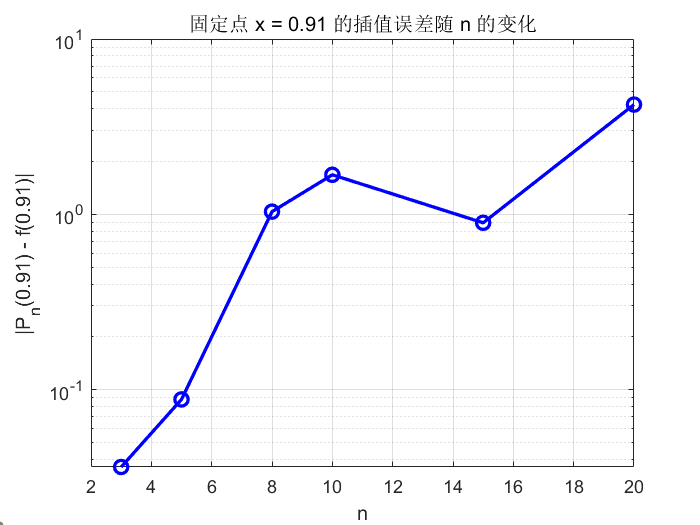
\includegraphics[width=0.7\textwidth]{固定点x=0.91的插值误差随n的变化.png}
    \caption{固定点 $x=0.91$ 的插值误差随 $n$ 的变化}
    \label{fig:fixed_point_error}
\end{figure}

根据实验结果, 在固定点 $x=0.91$ 处, 随着插值节点数 $n$ 的增加, Lagrange插值多项式的计算误差整体呈震荡上升趋势, 展现出等距节点高次插值的典型病态特征. 当 $n=3$ 和 $n=5$ 时, 误差均处于 $10^{-2}$ 量级, 尚可接受; 然而从 $n=8$ 开始, 误差显著增大至约 $1.035$, 到 $n=10$ 时进一步上升至 $1.680$, 插值结果已严重偏离真值. 值得关注的是, 当 $n=15$ 时误差反而略降至 $0.894$, 随后在 $n=20$ 时又跃升至 $4.225$, 这种非单调的起伏现象说明Runge振荡在不同多项式阶数下具有不同的相位与幅度, 使得同一固定点可能落在误差曲线的波峰或波谷. 但从整体量级看, 最大误差已超过 $4$, 远大于低次情形, 可见插值多项式在区间端点附近已出现发散趋势. 这一结果再次印证了Runge现象的典型特征: 对于函数 $f(x)=1/(1+25x^2)$, 等距节点的高次插值不仅无法提高逼近精度, 反而会导致端点附近的剧烈振荡, 且随着 $n$ 的增大, 插值结果在量级上不断恶化. 因此, 在实际计算中应避免简单增加等距节点数目, 而应采用切比雪夫节点分布或分段低次插值等策略, 以有效抑制Runge现象, 保证多项式插值的数值稳定性. 

\noindent{\bfseries 任务2}

\begin{figure}[htbp]
    \centering
    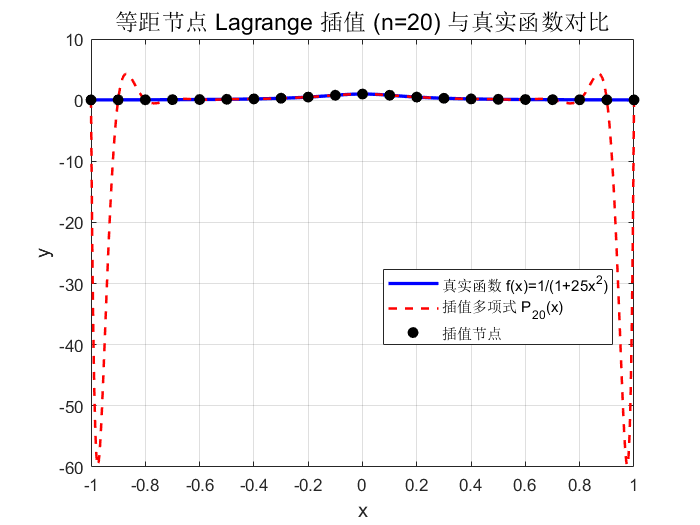
\includegraphics[width=0.8\textwidth]{等距节点Lagrange插值与真实函数对比.png}
    \caption{等距节点 Lagrange 插值与真实函数对比(n=20)}
    \label{fig:spaced_nodes_comparison}
\end{figure}
\begin{figure}[htbp]
    \centering
    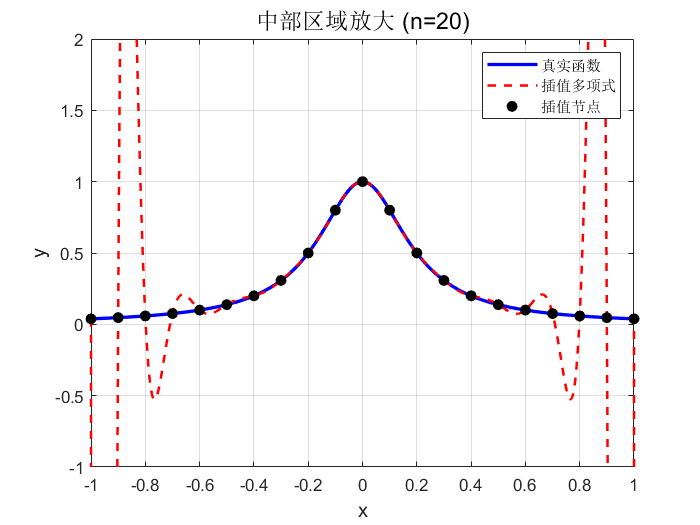
\includegraphics[width=0.8\textwidth]{中部区域放大.png}
    \caption{等距节点 Lagrange 插值与真实函数对比(中部区域放大) (n=20)}
    \label{fig:middle_region_zoom}
\end{figure}

如图\ref{fig:spaced_nodes_comparison}和图\ref{fig:middle_region_zoom}所示, 当取 $n=20$ 时, 绘制插值多项式 $P_{20}(x)$ 与真实函数 $f(x)=\frac{1}{1+25x^2}$ 的曲线进行对比, 可以清晰地观察到经典的Runge现象. 在区间中部, 特别是在 $x=0$ 附近, 插值曲线与真实函数较为接近, 能够基本反映函数的形态; 然而一旦靠近区间的两端(如 $x$ 接近 $-1$ 或 $1$), $P_{20}(x)$ 便出现剧烈的上下振荡, 幅度远远偏离实际函数值, 甚至在某些点处绝对值达到 $10^5$ 量级, 完全失去了逼近意义. 与平滑的 $f(x)$ 曲线相比, $P_{20}(x)$ 在端点附近呈现出高频、大幅度的摆动, 且这种振荡并不随着节点的进一步加密而减弱, 反而愈演愈烈. 这一对比直观地说明: 对于等距节点的高次多项式插值, 增加插值点数并不能带来精度的整体提升, 反而会在边界区域产生灾难性的数值发散, 这正是Runge现象最典型的几何表现. 因此, 在实际数值逼近中, 必须放弃单纯依靠增加等距节点来提高精度的做法, 转而采用Chebyshev节点分布或分段低次插值以消除边界振荡, 从而获得稳定、可靠的插值结果. 



\end{document}
